\chapter{Hidden Yet Quantifiable: A Lower Bound for Confounding Strength Using Randomized Trials}
\label{chap:confounding-test}
\chaptermark{Quantifying Hidden Confounding}

\chapterabstract{In the era of fast-paced precision medicine, observational studies play a major role in properly evaluating new treatments in clinical practice. Yet unobserved confounding can significantly compromise causal conclusions drawn from non-randomized data. This chapter develops a strategy that leverages randomized trials to quantify unobserved confounding. First, it designs a statistical test to detect unobserved confounding above a certain strength. Then, it uses the test to estimate an asymptotically valid lower bound on the true confounding strength. The chapter evaluates the power and validity of the test on synthetic and semi-synthetic datasets, and shows how the lower bound can identify the absence or presence of practically important unobserved confounding in a real-world example.}

\chapterpublication
  {This chapter is based on joint work co-led by the author of this thesis and appeared as:}
  {Piersilvio De Bartolomeis\equalcontributionmark, Javier Abad\equalcontributionmark, Konstantin Donhauser, and Fanny Yang (2024). ``Hidden yet quantifiable: A lower bound for confounding strength using randomized trials.'' In \emph{International Conference on Artificial Intelligence and Statistics}. \equalcontributionnote\ Source code is available at \url{https://github.com/jaabmar/confounder-lower-bound}.}
% TODO: Add personal contribution breakdown between Javier Abad and Piersilvio De Bartolomeis.

\vspace{-0.6\baselineskip}

\section{Motivation and Scope}

Building on the causal inference and sensitivity analysis preliminaries in Chapter~\ref{chap:background}, this chapter asks whether observational datasets support valid causal conclusions before they are acted upon or shared. In high-stakes domains such as healthcare, observational treatment-effect estimates can fail whenever unobserved confounders bias treatment assignment. This chapter therefore uses randomized trials and marginal sensitivity analysis to quantify the strength of such hidden confounding.

Monitoring the performance of a newly approved treatment is crucial, a process commonly referred to as post-marketing surveillance \citep{vlahovic2011postmarketing}. Nowadays, regulatory and clinical practice increasingly integrate observational data in this process to address the shortcomings of randomized evidence \citep{platt2018fda,klonoff2020new}. This strategy is essential for validating personalized and high-cost treatments, such as immunotherapy for some cancers, where randomized evidence may be scarce and treatment costs substantial \citep{goetz2018personalized}.

Yet unobserved confounding can significantly compromise causal conclusions drawn from observational data. Sensitivity analysis has been the prevalent paradigm for reasoning about this issue since the work of \citet{cornfield59}. This field studies how a specified strength of unobserved confounding affects causal conclusions and introduces the concept of a critical value \citep{vanderweele2017sensitivity,jin2023sensitivity}: the minimum strength unobserved confounders would need to have to explain away the estimated treatment effect. However, critical values are solely based on observational data and can differ substantially from the true confounding strength. As a result, practitioners often still rely on heuristic judgments to decide whether an observational study is flawed.

Estimating the true confounding strength is infeasible without further assumptions. Yet, once a treatment gains approval, a randomized trial may be available and can enable more effective strategies to address unobserved confounding. This chapter proposes such a strategy: using randomized trials to test and quantify the true confounding strength. If strong confounding is detected, practitioners can take proactive measures, most directly by identifying and incorporating relevant covariates that were initially overlooked \citep{dreyer2018advancing}. If only small confounding is detected, the observational analysis may remain informative. Figure~\ref{fig:confounding-motivating-example} illustrates this role in the drug-evaluation pipeline.

The method introduced in this chapter has three main components:
\begin{itemize}
  \item \textit{Testing confounding above a specified strength.} We introduce statistical tests to detect unobserved confounding above a certain strength.
  \item \textit{Lower bounding the true confounding strength.} We show how these tests can be used to estimate an asymptotically valid lower bound on the true confounding strength.
  \item \textit{Empirical validation and real-world application.} We evaluate the finite-sample validity and power of the tests on synthetic and semi-synthetic datasets, and use the Women's Health Initiative to show how the lower bound distinguishes negligible from practically important confounding.
\end{itemize}

The rest of the chapter first positions the approach, then introduces the setting and sensitivity model, constructs and inverts the tests, and reports the empirical evaluation. Appendix~\ref{chap:appendix-confounding-test} contains proof details, nested-design notes, sensitivity-model discussion, experimental details, and additional experiments.

\begin{figure}[!t]
  \centering
  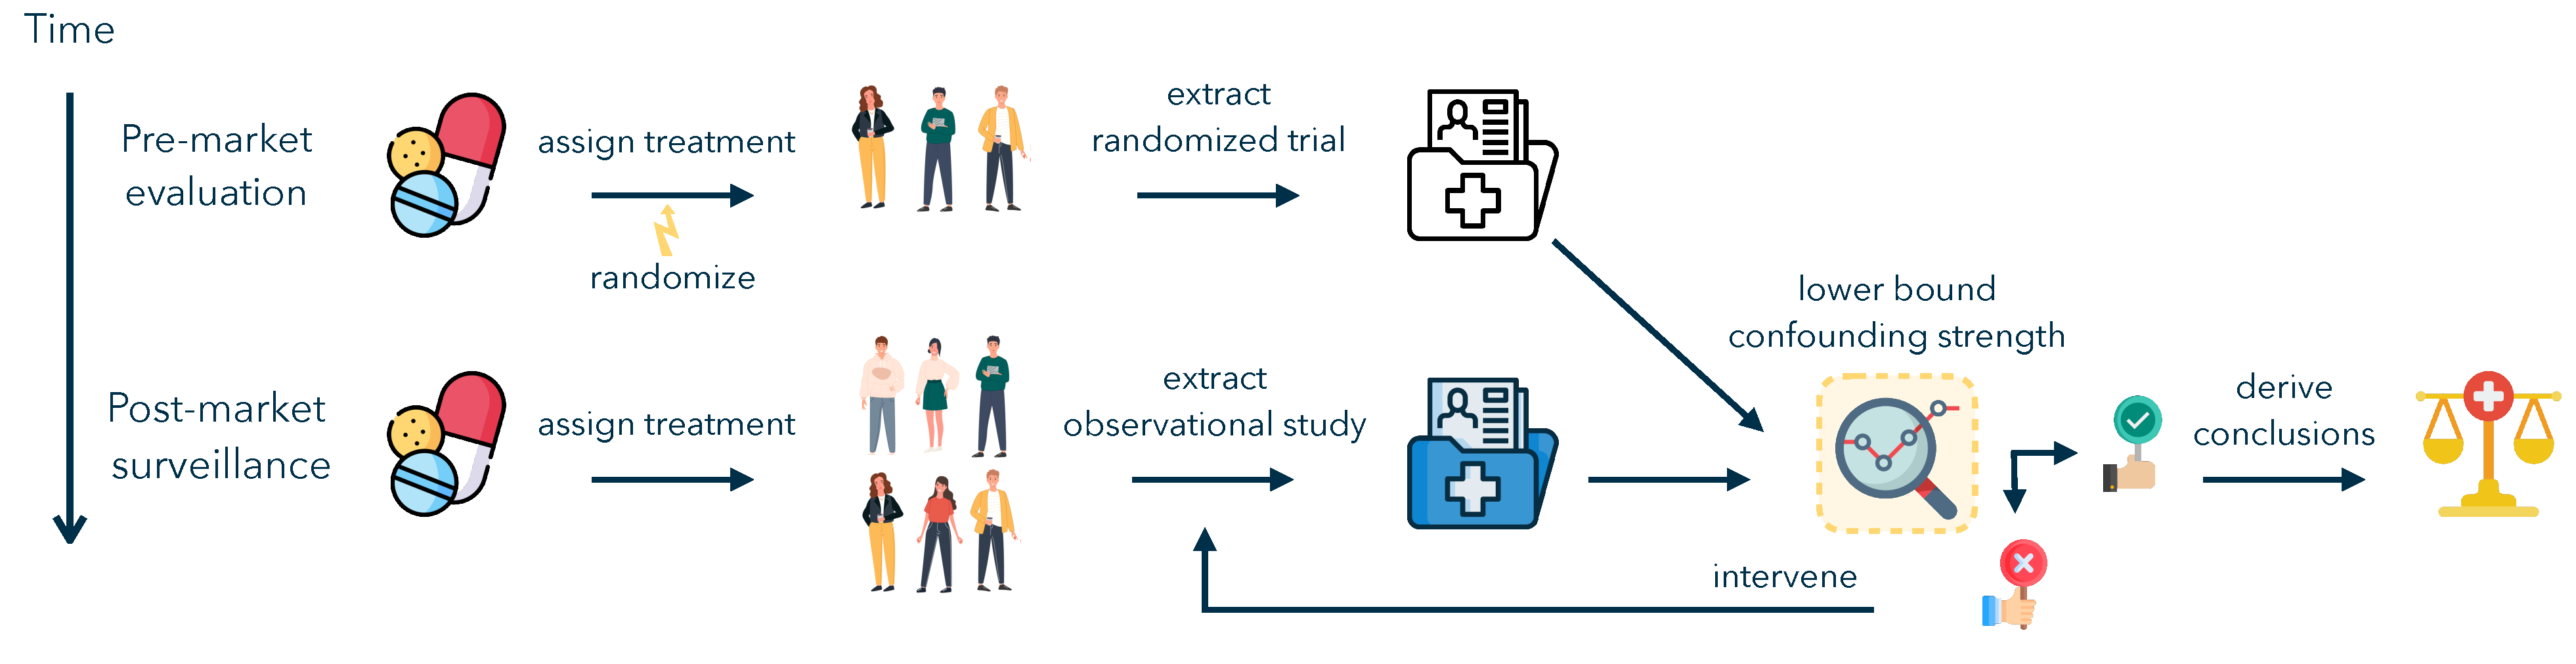
\includegraphics[width=0.82\textwidth]{papers/confounding_test/figures/motivating_example.pdf}
  \caption{Illustrative role of the proposed lower bound in post-marketing evaluation. Randomized evidence helps decide whether an observational study is compatible with small hidden confounding or should trigger corrective action.}
  \label{fig:confounding-motivating-example}
\end{figure}

\section{Positioning Relative to Existing Methods}

Sensitivity analysis is the classical framework for reasoning about hidden confounding in observational causal inference, dating back to the work of \citet{cornfield59}. Modern sensitivity analyses typically ask how strong an unobserved confounder would need to be to change a substantive causal conclusion, often summarized through a critical value \citep{vanderweele2017sensitivity,jin2023sensitivity}. Such critical values are useful robustness diagnostics, but they are computed from observational data alone. They describe how much confounding would be sufficient to alter a conclusion, rather than how much hidden confounding is actually present.

A related line of work designs tests for the presence of unobserved confounding. Several such tests use randomized trials as a reference point and compare treatment-effect estimates obtained from randomized and observational data \citep{viele2014use,hussain2022falsification,yangelastic}. Extensions test for discrepancies in conditional treatment-effect estimates or adapt the testing problem to censored outcomes \citep{hussain2023falsification,demirel2024benchmarking}. Other approaches use instrumental variables, negative controls, or multiple observational studies to detect violations of the unconfoundedness assumption \citep{lipsitch2010negative,de2014testing,donald2014testing,karlsson2023detecting}. These tests answer an important but binary question: whether hidden confounding can be detected. In many applications, this question is too stringent: residual confounding may be expected and may not invalidate the practical conclusion of a study. 

Another line of work calibrates the value of the confounding strength using only observational data \citep{hsu2013calibrating,veitch2020sense}. Such calibration can help interpret robustness values, but the calibrated strength may still differ arbitrarily from the true confounding strength, even with infinite samples.

The approach in this chapter sits between these directions. Like sensitivity analysis, it works with a quantitative notion of confounding strength. Like tests based on randomized trials, it uses randomized evidence to diagnose confounding. Its distinctive contribution is to move beyond detecting whether any hidden confounding is present: the chapter tests whether confounding exceeds a specified strength and then inverts those tests to obtain a lower bound on the true confounding strength.

\section{Problem Setting and Preliminaries}
\label{sec:confounding-setting}

We have access to data from a randomized trial, denoted by \(\mathrm{rct}\), and an observational study, denoted by \(\mathrm{os}\). These two data sources come from underlying full distributions. For each source \(\diamond \in \{\mathrm{rct},\mathrm{os}\}\), we write
\[
  \mathbb{P}^{\diamond}_{\mathrm{full}}
\]
for an underlying full distribution over
\[
  \bigl(X,U,Y(0),Y(1),Y,T\bigr).
\]
Here \(X \in \RR^d\) denotes observed covariates, \(U \in \RR^k\) denotes unobserved confounders, \(Y(0)\) and \(Y(1)\) are bounded potential outcomes, \(Y \in \RR\) is the observed outcome, and \(T \in \{0,1\}\) is the treatment indicator. The variable \(U\) and the potential outcomes are never directly observed. We only observe samples from the marginals
\[
  \mathbb{P}^{\mathrm{rct}}
  =
  \mathcal{M}\bigl(\mathbb{P}^{\mathrm{rct}}_{\mathrm{full}}\bigr),
  \qquad
  \mathbb{P}^{\mathrm{os}}
  =
  \mathcal{M}\bigl(\mathbb{P}^{\mathrm{os}}_{\mathrm{full}}\bigr),
\]
where \(\mathcal{M}\) denotes marginalization to \((X,Y,T)\).

We assume that the full distribution can be factorized as follows for the randomized trial and observational study:
\begin{equation}
\label{eq:confounding-factorization}
  \mathbb{P}^{\diamond}_{\mathrm{full}}
  =
  \underbrace{\mathbb{P}_{Y\mid Y(1),Y(0),T}}_{\mathbb{P}_{\mathrm{det}}}
  \underbrace{\mathbb{P}_{Y(1),Y(0)\mid X,U}}_{\mathbb{P}_{\mathrm{inv}}}
  \underbrace{\mathbb{P}^{\diamond}_{X,T,U}}_{\mathbb{P}^{\diamond}_{\mathrm{cnf}}}.
\end{equation}
Here \(\mathbb{P}_{\mathrm{det}}\) is given by \(Y=Y(T)\), \(\mathbb{P}_{\mathrm{inv}}\) is invariant across studies, and \(\mathbb{P}^{\diamond}_{\mathrm{cnf}}\) may differ for \(\diamond \in \{\mathrm{rct},\mathrm{os}\}\). This factorization captures the essence of the potential-outcome framework while allowing shifts in the marginal distribution of observed and unobserved confounders. Figure~\ref{fig:confounding-dag} gives the corresponding graphical intuition; it is only an illustration and is not used as a formal graphical-model assumption.

\begin{figure}[!t]
  \centering
  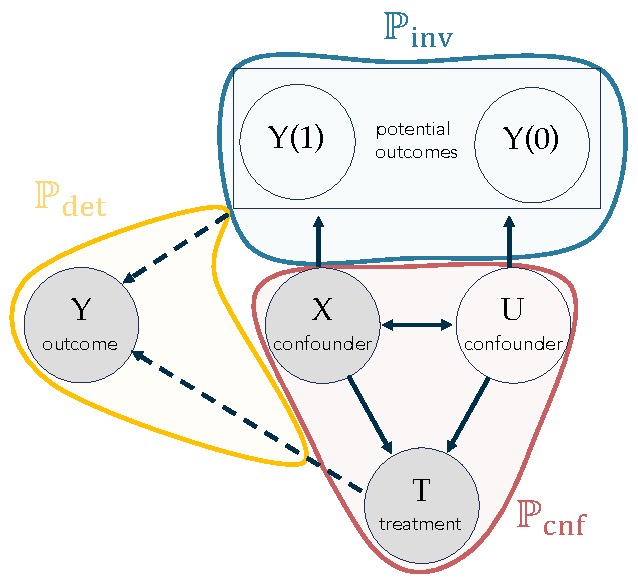
\includegraphics[width=0.54\textwidth]{papers/confounding_test/figures/dag.pdf}
  \caption{Graphical intuition for the randomized-trial and observational-study setting. The invariant outcome mechanism is shared across sources, while the source-specific confounding mechanism may change. In the randomized trial, internal validity removes the arrow from the confounders \((X,U)\) to treatment \(T\). Observed variables are shaded.}
  \label{fig:confounding-dag}
\end{figure}

We now introduce three additional assumptions required for the validity of the statistical tests and the resulting lower bound. First, we require transportability of the conditional average treatment effect (CATE).

\begin{assumption}[Transportability]
\label{asm:confounding-transportability}
The conditional average treatment effect is invariant across the randomized trial and the observational study:
\[
  \mathbb{E}_{\mathbb{P}^{\mathrm{os}}_{\mathrm{full}}}
  \bigl[Y(1)-Y(0)\mid X\bigr]
  =
  \mathbb{E}_{\mathbb{P}^{\mathrm{rct}}_{\mathrm{full}}}
  \bigl[Y(1)-Y(0)\mid X\bigr].
\]
\end{assumption}

This property is standard for generalizing the findings of randomized trials to another population \citep{o2014generalizing,colnet2020causal,degtiar2023review}, and is weaker than ignorability of study selection \citep{sugden1984ignorable,hotz2005predicting} or sample ignorability of treatment effects \citep{kern2016assessing}.

The second assumption is the source of identification in the randomized trial.

\begin{assumption}[Internal validity]
\label{asm:confounding-internal-validity}
In the randomized trial, treatment is assigned independently of observed and unobserved covariates:
\[
  \mathbb{P}^{\mathrm{rct}}_{X,T,U}
  =
  \mathbb{P}^{\mathrm{rct}}_T
  \mathbb{P}^{\mathrm{rct}}_{X,U},
  \qquad
  \mathbb{P}^{\mathrm{rct}}(T=1)=\pi\in(0,1).
\]
\end{assumption}

Internal validity holds by design in a completely randomized experiment, allowing for unbiased estimation of the treatment effect. Observational studies, on the other hand, can have arbitrary confounding structures reflected in \(\mathbb{P}^{\mathrm{os}}_{X,T,U}\).

The third assumption ensures that the observational study can support the comparisons made with randomized evidence.

\begin{assumption}[Support inclusion]
\label{asm:confounding-support-inclusion}
The covariate support of the randomized trial is contained in the covariate support of the observational study:
\[
  \supp\bigl(\mathbb{P}^{\mathrm{rct}}_X\bigr)
  \subseteq
  \supp\bigl(\mathbb{P}^{\mathrm{os}}_X\bigr).
\]
\end{assumption}

This assumption is strictly weaker than positivity of trial participation \citep{stuart2011use,hartman2015sample,andrews2017weighting,nie2021covariate,colnet2022reweighting}. It is also expected to hold in the setting considered here, since it aligns with the design of observational studies by regulatory agencies for drug monitoring \citep{he2020clinical}, and particularly for post-marketing surveillance \citep{franklin2019evaluating,schurman2019framework}.

\paragraph{Sensitivity analysis.}
Sensitivity analysis is commonly used to account for unobserved confounding in observational data. In particular, it estimates an interval for the treatment effect that depends on an assumed confounding strength \(\Gamma\). Throughout the chapter, the confounding strength is defined using the marginal sensitivity model \citep{tan2006distributional}. For \(\Gamma \geq 1\), define \(\mathcal{E}(\Gamma)\) as the set of confounding mechanisms whose treatment odds satisfy the constraint
\[
  \frac{1}{\Gamma}
  \leq
  \frac{
    \mathbb{P}_{\mathrm{cnf}}(T=1\mid X,U)/
    \mathbb{P}_{\mathrm{cnf}}(T=0\mid X,U)
  }{
    \mathbb{P}_{\mathrm{cnf}}(T=1\mid X)/
    \mathbb{P}_{\mathrm{cnf}}(T=0\mid X)
  }
  \leq
  \Gamma
  \qquad\text{almost surely.}
\]
When \(\Gamma=1\), the treatment odds cannot depend on \(U\) after conditioning on \(X\), corresponding to no hidden confounding under this model. Larger values of \(\Gamma\) allow stronger deviations between the full propensity score and the observed propensity score.

Under this notion of confounding strength, we can define a set of full distributions that are compatible with the marginal distribution of the observational study and have bounded odds ratio.
\begin{definition}[Marginal sensitivity set]
\label{def:confounding-msm}
For \(\Gamma \geq 1\), the set \(\mathcal{E}(\mathbb{P}^{\mathrm{os}},\Gamma)\) consists of all full distributions
\[
  \widetilde{\mathbb{P}}_{\mathrm{full}}
  =
  \mathbb{P}_{\mathrm{det}}
  \widetilde{\mathbb{P}}_{\mathrm{inv}}
  \widetilde{\mathbb{P}}_{\mathrm{cnf}}
\]
such that \(\widetilde{\mathbb{P}}_{\mathrm{cnf}}\in\mathcal{E}(\Gamma)\) and
\[
  \mathcal{M}\bigl(
  \mathbb{P}_{\mathrm{det}}
  \widetilde{\mathbb{P}}_{\mathrm{inv}}
  \widetilde{\mathbb{P}}_{\mathrm{cnf}}
  \bigr)
  =
  \mathbb{P}^{\mathrm{os}}.
\]
\end{definition}
In other words, this set contains all the full distributions that could have induced the marginal distribution of the observational study \(\mathbb{P}^{\mathrm{os}}\).

Since the marginal sensitivity set contains the true observational full distribution if \(\Gamma\) is well specified, we can partially identify the conditional treatment effect as follows.
\begin{definition}[Sensitivity bounds]
\label{def:confounding-sensitivity-bounds}
For a full distribution \(\mathbb{P}_{\mathrm{full}}\), define the conditional average treatment effect
\[
  \mu(X,\mathbb{P}_{\mathrm{full}})
  =
  \mathbb{E}_{\mathbb{P}_{\mathrm{full}}}
  \bigl[Y(1)-Y(0)\mid X\bigr].
\]
The lower and upper CATE bounds under confounding strength \(\Gamma\) are
\[
  \mu^-_{\Gamma}(X)
  =
  \inf_{\widetilde{\mathbb{P}}_{\mathrm{full}}
  \in
  \mathcal{E}(\mathbb{P}^{\mathrm{os}},\Gamma)}
  \mu(X,\widetilde{\mathbb{P}}_{\mathrm{full}}),
  \qquad
  \mu^+_{\Gamma}(X)
  =
  \sup_{\widetilde{\mathbb{P}}_{\mathrm{full}}
  \in
  \mathcal{E}(\mathbb{P}^{\mathrm{os}},\Gamma)}
  \mu(X,\widetilde{\mathbb{P}}_{\mathrm{full}}).
\]
For a target covariate distribution \(\mathbb{P}_X\), define the average treatment effect (ATE) as
\[
  \mu(\mathbb{P}_X,\mathbb{P}_{\mathrm{full}})
  =
  \mathbb{E}_{\mathbb{P}_X}
  \bigl[\mu(X,\mathbb{P}_{\mathrm{full}})\bigr],
\]
and the corresponding ATE bounds
\[
  \mu^-_{\Gamma}(\mathbb{P}_X)
  =
  \mathbb{E}_{\mathbb{P}_X}\bigl[\mu^-_{\Gamma}(X)\bigr],
  \qquad
  \mu^+_{\Gamma}(\mathbb{P}_X)
  =
  \mathbb{E}_{\mathbb{P}_X}\bigl[\mu^+_{\Gamma}(X)\bigr].
\]
\end{definition}

Several estimators are available for these CATE and ATE sensitivity bounds \citep{kallus2019interval,zhao2019sensitivity,jesson2021quantifying,dorn2021doubly,dorn2022sharp,oprescu2023b}. The testing procedure treats such estimators as inputs. For the present chapter, the key point is the implication they provide: if the proposed value \(\Gamma\) is large enough to contain the true hidden confounding, then the randomized target effect should fall inside the corresponding observational sensitivity interval.

\section{Sensitivity Analysis as a Testing Problem}
\label{sec:confounding-testing-problem}

We would like to test whether the unobserved full distribution \(\mathbb{P}^{\mathrm{os}}_{\mathrm{full}}\), which marginalizes to the observational distribution \(\mathbb{P}^{\mathrm{os}}\), has confounding strength at most \(\Gamma\). This is captured by the null hypothesis
\[
  H_0(\Gamma):
  \mathbb{P}^{\mathrm{os}}_{\mathrm{full}}
  \in
  \mathcal{E}(\mathbb{P}^{\mathrm{os}},\Gamma).
\]
Rejecting \(H_0(\Gamma)\) provides evidence that the hidden confounding strength exceeds \(\Gamma\). When \(\Gamma=1\), the problem reduces to testing whether there are no unobserved confounders under the marginal sensitivity model. This special case is the binary testing problem studied in much of the prior work on detecting unobserved confounding.

In real-world scenarios, binary tests can be overly stringent because they invalidate an observational study even when the unobserved confounding is negligible. To overcome this limitation, the chapter studies the more general case \(\Gamma>1\). The underlying observation is simple: when \(H_0(\Gamma)\) is true, the average treatment effect under a target population should fall between the valid lower and upper sensitivity bounds constructed from the observational study. A randomized trial can estimate such a target effect under the assumptions above.

\begin{lemma}
\label{lem:confounding-testing-observation}
Let \(\mathbb{P}_X\) be any target covariate distribution satisfying
\[
  \supp(\mathbb{P}_X)
  \subseteq
  \supp(\mathbb{P}^{\mathrm{os}}_X).
\]
Let \(\mathbb{P}_{\mathrm{full}}\) be any full distribution satisfying
\[
  \mu(X,\mathbb{P}_{\mathrm{full}})
  =
  \mu(X,\mathbb{P}^{\mathrm{os}}_{\mathrm{full}})
\]
on \(\supp(\mathbb{P}_X)\).
If \(H_0(\Gamma)\) holds, then
\[
  \mu(\mathbb{P}_X,\mathbb{P}_{\mathrm{full}})
  \in
  \bigl[
    \mu^-_{\Gamma}(\mathbb{P}_X),
    \mu^+_{\Gamma}(\mathbb{P}_X)
  \bigr].
\]
\end{lemma}

In this chapter, \(\mathbb{P}_{\mathrm{full}}\) is instantiated using the randomized trial, and \(\mathbb{P}_X\) is chosen as a target covariate distribution for which the treatment effect can be estimated from randomized data. The lemma is therefore the bridge from sensitivity analysis to statistical testing: under \(H_0(\Gamma)\), the randomized target effect should be compatible with the sensitivity interval implied by the observational study. The corresponding proof is recorded in Appendix~\ref{app:confounding-proof-compatibility}.

\section{Testing for Confounding Above a Given Strength}
\label{sec:confounding-methodology}

In what follows, we have access to a randomized trial
\[
  D_{\mathrm{rct}}
  =
  \{(X_i,Y_i,T_i)\}_{i=1}^{n_{\mathrm{rct}}}
\]
sampled i.i.d. from \(\mathbb{P}^{\mathrm{rct}}\), and an observational study
\[
  D_{\mathrm{os}}
  =
  \{(X_i,Y_i,T_i)\}_{i=1}^{n_{\mathrm{os}}}
\]
sampled i.i.d. from \(\mathbb{P}^{\mathrm{os}}\). We first propose estimates for the average treatment effect under two target populations. Then, we leverage these estimates together with the sensitivity bounds to design asymptotically valid tests at significance level \(\alpha\). Finally, we show in the next section how such tests can be used to establish an asymptotically valid lower bound on the unobserved confounding strength.

\paragraph{Estimating the ATE.}
We discuss here how the average treatment effect can be estimated using data from the randomized trial. First, define a target covariate population \(\mathbb{P}^{\star}_X\) for the ATE. We use two such targets: the randomized-trial population \(\mathbb{P}^{\mathrm{rct}}_X\), and the observational population restricted to the support of the randomized trial,
\[
  \mathbb{P}^{\widetilde{\mathrm{os}}}_X
  =
  \mathbb{P}^{\mathrm{os}}_X
  \bigm|
  X \in \supp(\mathbb{P}^{\mathrm{rct}}_X).
\]
The second target is useful when the corresponding shift from the trial population can be estimated or identified; nested trial designs provide one setting where these weights are naturally available. For \(\star \in \{\mathrm{rct},\widetilde{\mathrm{os}}\}\), when \(\mathbb{P}^{\star}_X\) is absolutely continuous with respect to the randomized-trial covariate distribution, define the reweighting function
\[
  w_{\star}(X)
  =
  \frac{d\mathbb{P}^{\star}_X}{d\mathbb{P}^{\mathrm{rct}}_X}(X),
\]
with \(w_{\mathrm{rct}}(X)=1\). Under the transportability, internal-validity, and support-inclusion assumptions, and with these weights well defined, the target ATE can be identified from the randomized trial as
\[
  \mu\bigl(\mathbb{P}^{\star}_X,\mathbb{P}^{\mathrm{os}}_{\mathrm{full}}\bigr)
  =
  \mu\bigl(\mathbb{P}^{\star}_X,\mathbb{P}^{\mathrm{rct}}_{\mathrm{full}}\bigr)
  =
  \mathbb{E}_{\mathbb{P}^{\mathrm{rct}}}
  \left[
    Y
    \left(
      \frac{T}{\pi}
      -
      \frac{1-T}{1-\pi}
    \right)
    w_{\star}(X)
  \right].
\]
This identification result is the standard transportability argument for estimating a target-population ATE from randomized data \citep{cole2010generalizing,colnet2023risk}; see Appendix~\ref{app:confounding-proof-ate} for the derivation. When the distribution shift between \(\mathbb{P}^{\mathrm{rct}}_X\) and \(\mathbb{P}^{\star}_X\) can be corrected by \(w_{\star}\), randomized outcomes identify the target effect. It gives the empirical estimate
\[
  \widehat{\mu}_{\star}
  =
  \frac{1}{n_{\mathrm{rct}}}
  \sum_{(X_i,Y_i,T_i)\in D_{\mathrm{rct}}}
    Y_i
    \left(
      \frac{T_i}{\pi}
      -
      \frac{1-T_i}{1-\pi}
    \right)
    w_{\star}(X_i),
\]
together with an estimate \(\widehat{\sigma}_{\star}^2\) of the sampling variance of \(\widehat{\mu}_{\star}\), equivalently the squared standard error used in the test statistic below.

\paragraph{Estimating the sensitivity interval.}
Next, we discuss how the sensitivity bounds
\[
  \mu^-_{\Gamma}(\mathbb{P}^{\star}_X),
  \qquad
  \mu^+_{\Gamma}(\mathbb{P}^{\star}_X)
\]
can be estimated using data from the observational study and the target population. Here, the approach varies based on the target population.
\begin{itemize}[leftmargin=*]
  \item For \(\mathbb{P}^{\star}_X=\mathbb{P}^{\mathrm{rct}}_X\), we estimate CATE sensitivity bounds from observational data and average them over the target population. In the experiments, we use the B-Learner \citep{oprescu2023b} for these CATE bounds.
  \item For \(\mathbb{P}^{\star}_X=\mathbb{P}^{\widetilde{\mathrm{os}}}_X\), there are two options: either estimate CATE sensitivity bounds and average them over the restricted observational population, or directly estimate ATE sensitivity bounds over the target population. In the experiments, we directly estimate these ATE bounds using either DVDS \citep{dorn2021doubly} or the QB estimator \citep{dorn2022sharp}.
\end{itemize}
We write the resulting estimates as
\[
  \widehat{\mu}^-_{\Gamma,\star},
  \qquad
  \widehat{\mu}^+_{\Gamma,\star},
\]
with sampling-variance estimates \((\widehat{\sigma}^-_{\Gamma,\star})^2\) and \((\widehat{\sigma}^+_{\Gamma,\star})^2\).
These methods yield estimates of the lower and upper endpoints used by the test. Nevertheless, the testing procedure itself is agnostic to the particular sensitivity-bound estimator, allowing various valid sensitivity-analysis methods to be adopted.

\paragraph{Two statistical tests.}
We outline the testing procedure in Algorithm~\ref{alg:confounding-test}, which can be instantiated for either target population. This results in two statistical tests, \(\widehat{\phi}_{\mathrm{rct}}\) and \(\widehat{\phi}_{\widetilde{\mathrm{os}}}\), for the null hypothesis \(H_0(\Gamma)\). The tests compare the randomized-trial estimate \(\widehat{\mu}_{\star}\) with the estimated sensitivity interval. If the randomized estimate is significantly below the lower endpoint or above the upper endpoint, then \(H_0(\Gamma)\) is rejected. Define
\[
  \widehat{T}^+_{\Gamma,\star}
  =
  \frac{
    \widehat{\mu}^+_{\Gamma,\star}
    -
    \widehat{\mu}_{\star}
  }{
    \widehat{s}^+_{\Gamma,\star}
  },
  \qquad
  \widehat{T}^-_{\Gamma,\star}
  =
  \frac{
    \widehat{\mu}_{\star}
    -
    \widehat{\mu}^-_{\Gamma,\star}
  }{
    \widehat{s}^-_{\Gamma,\star}
  },
\]
where \(\widehat{s}^+_{\Gamma,\star}\) and \(\widehat{s}^-_{\Gamma,\star}\) are standard errors for the endpoint-effect differences. For the two target populations, we use
\[
  \widehat{s}^\pm_{\Gamma,\mathrm{rct}}
  =
  \sqrt{
    (\widehat{\sigma}^\pm_{\Gamma,\mathrm{rct}})^2
    +
    \widehat{\sigma}_{\mathrm{rct}}^2
    +
    2\widehat{\sigma}^\pm_{\Gamma,\mathrm{rct}}\widehat{\sigma}_{\mathrm{rct}}
  },
  \qquad
  \widehat{s}^\pm_{\Gamma,\widetilde{\mathrm{os}}}
  =
  \sqrt{
    (\widehat{\sigma}^\pm_{\Gamma,\widetilde{\mathrm{os}}})^2
    +
    \widehat{\sigma}_{\widetilde{\mathrm{os}}}^2
  }.
\]
For the trial-targeted test, the extra cross term is a conservative covariance bound for the shared randomized-trial covariates. For the restricted-observational test, the randomized target-effect estimate and the directly estimated observational ATE bounds are treated as independent sample contributions.
The resulting level-\(\alpha\) test is
\[
  \widehat{\phi}_{\star}(\Gamma,\alpha)
  =
  \mathbf{1}
  \left\{
    \min\bigl(
      \widehat{T}^+_{\Gamma,\star},
      \widehat{T}^-_{\Gamma,\star}
    \bigr)
    <
    z_{\alpha/2}
  \right\},
\]
where \(z_{\alpha/2}=\Phi^{-1}(\alpha/2)\) is the lower \(\alpha/2\)-quantile of the standard normal distribution. Instantiating \(\star=\mathrm{rct}\) gives the test \(\widehat{\phi}_{\mathrm{rct}}\), while \(\star=\widetilde{\mathrm{os}}\) gives the test \(\widehat{\phi}_{\widetilde{\mathrm{os}}}\).

\begin{algorithm}[t]
  \caption{Statistical test for detecting unobserved confounding}
  \label{alg:confounding-test}
  \centering
  \fbox{
    \begin{minipage}{0.92\textwidth}
      \textbf{Inputs:} target \(\star\in\{\mathrm{rct},\widetilde{\mathrm{os}}\}\), datasets \(D_{\mathrm{rct}}\) and \(D_{\mathrm{os}}\), significance level \(\alpha\in(0,1)\), and confounding strength \(\Gamma\geq 1\).
      \begin{enumerate}
        \item \textbf{Choose target:} set \(\mathbb{P}^{\star}_X\) and specify (or estimate, when unknown) the corresponding importance weights \(w_{\star}\).
        \item \textbf{Estimate randomized target effect:} compute \(\widehat{\mu}_{\star}\) from \(D_{\mathrm{rct}}\) using inverse treatment-probability weighting and \(w_{\star}\), together with a consistent sampling-variance estimate \(\widehat{\sigma}_{\star}^2\).
        \item \textbf{Estimate sensitivity interval:} use \(D_{\mathrm{os}}\) to estimate \(\widehat{\mu}^-_{\Gamma,\star}\) and \(\widehat{\mu}^+_{\Gamma,\star}\) over \(\mathbb{P}^{\star}_X\), together with consistent sampling-variance estimates \((\widehat{\sigma}^-_{\Gamma,\star})^2\) and \((\widehat{\sigma}^+_{\Gamma,\star})^2\).
        \item \textbf{Compare:} form the one-sided statistics \(\widehat{T}^+_{\Gamma,\star}\) and \(\widehat{T}^-_{\Gamma,\star}\) using \(\widehat{s}^{\pm}_{\Gamma,\star}\).
        \item \textbf{Reject:} output \(\widehat{\phi}_{\star}(\Gamma,\alpha)=\mathbf{1}\bigl\{\min(\widehat{T}^+_{\Gamma,\star},\widehat{T}^-_{\Gamma,\star})<z_{\alpha/2}\bigr\}\).
      \end{enumerate}
    \end{minipage}
  }
\end{algorithm}

\begin{proposition}[Validity of the tests]
\label{prop:confounding-test-validity}
Fix \(\Gamma\geq 1\) and \(\alpha\in(0,1)\). Under the setting of Section~\ref{sec:confounding-setting} and Assumptions~\ref{asm:confounding-transportability}--\ref{asm:confounding-support-inclusion}, suppose the sampling-variance estimators in Algorithm~\ref{alg:confounding-test} are consistent with respect to the asymptotic variances \(\sigma_{\star}^2\) and \((\sigma^{\pm}_{\Gamma,\star})^2\) defined in Appendix~\ref{app:confounding-proof-tests}, namely \(n_{\mathrm{rct}}\widehat{\sigma}_{\star}^2 \xrightarrow{p} \sigma_{\star}^2\) for \(\star\in\{\mathrm{rct},\widetilde{\mathrm{os}}\}\), \(n_{\mathrm{rct}}(\widehat{\sigma}^{\pm}_{\Gamma,\mathrm{rct}})^2 \xrightarrow{p} (\sigma^{\pm}_{\Gamma,\mathrm{rct}})^2\), and \(n_{\mathrm{os}}(\widehat{\sigma}^{\pm}_{\Gamma,\widetilde{\mathrm{os}}})^2 \xrightarrow{p} (\sigma^{\pm}_{\Gamma,\widetilde{\mathrm{os}}})^2\). Then the tests in Algorithm~\ref{alg:confounding-test} are asymptotically valid for \(H_0(\Gamma)\) under the following regularity conditions:
\begin{enumerate}
  \item If \(n_{\mathrm{rct}}/n_{\mathrm{os}}\to 0\) and the estimated CATE sensitivity bounds satisfy
  \[
    \bigl\|
      \widehat{\mu}^{\pm}_{\Gamma}(\cdot)
      -
      \mu^{\pm}_{\Gamma}(\cdot)
    \bigr\|_{L^2(\mathbb{P}^{\mathrm{rct}}_X)}
    =
    O_{\mathbb{P}}(n_{\mathrm{os}}^{-1/2}),
  \]
  then \(\widehat{\phi}_{\mathrm{rct}}(\Gamma,\alpha)\) is an asymptotically valid level-\(\alpha\) test.
  \item If \(n_{\mathrm{rct}}/(n_{\mathrm{rct}}+n_{\mathrm{os}})\to\rho\in(0,1)\), \(\mathbb{E}_{\mathbb{P}^{\mathrm{rct}}}[w_{\widetilde{\mathrm{os}}}(X)^2]<\infty\), and the estimated ATE sensitivity bounds are consistent and satisfy
  \[
  \begin{aligned}
    \sqrt{n_{\mathrm{os}}}
    \bigl(
      \widehat{\mu}^{+}_{\Gamma,\widetilde{\mathrm{os}}}
      -
      \mu^{+}_{\Gamma}(\mathbb{P}^{\widetilde{\mathrm{os}}}_X)
    \bigr)
    &\xrightarrow{d}
    \mathcal{N}\bigl(0,(\sigma^{+}_{\Gamma,\widetilde{\mathrm{os}}})^2\bigr), \\
    \sqrt{n_{\mathrm{os}}}
    \bigl(
      \widehat{\mu}^{-}_{\Gamma,\widetilde{\mathrm{os}}}
      -
      \mu^{-}_{\Gamma}(\mathbb{P}^{\widetilde{\mathrm{os}}}_X)
    \bigr)
    &\xrightarrow{d}
    \mathcal{N}\bigl(0,(\sigma^{-}_{\Gamma,\widetilde{\mathrm{os}}})^2\bigr),
  \end{aligned}
  \]
  then \(\widehat{\phi}_{\widetilde{\mathrm{os}}}(\Gamma,\alpha)\) is an asymptotically valid level-\(\alpha\) test.
\end{enumerate}
That is, in either case,
\[
  \limsup_{n_{\mathrm{rct}},n_{\mathrm{os}}\to\infty}
  \mathbb{P}_{H_0(\Gamma)}
  \bigl(
    \widehat{\phi}_{\star}(\Gamma,\alpha)=1
  \bigr)
  \leq
  \alpha.
\]
\end{proposition}

The full proof is reserved for Appendix~\ref{app:confounding-proof-tests}. It is based on asymptotic normality of the randomized target-effect estimator and the estimated sensitivity endpoints. Notably, the condition for \(\widehat{\phi}_{\widetilde{\mathrm{os}}}\), together with the fixed limiting proportions of the randomized trial and observational study, is relatively mild and expected to hold for a range of ATE sensitivity-bound estimators, including DVDS \citep{dorn2021doubly}. On the other hand, the condition for \(\widehat{\phi}_{\mathrm{rct}}\) is stronger and generally expected to hold only when \(n_{\mathrm{os}}\gg n_{\mathrm{rct}}\).

In essence, the two tests work under different estimation assumptions: \(\widehat{\phi}_{\mathrm{rct}}\) relies on a consistent estimate of the CATE sensitivity bounds, while \(\widehat{\phi}_{\widetilde{\mathrm{os}}}\) relies on directly estimating the ATE sensitivity bounds together with the importance weights \(w_{\widetilde{\mathrm{os}}}\). Proposition~\ref{prop:confounding-test-validity}(2) treats \(w_{\widetilde{\mathrm{os}}}\) as known for the theoretical guarantee; in practice, the importance weights can be identified and estimated when the observational study and randomized trial follow a nested trial design \citep{olschewski1985comprehensive,olschewski1992analysis,choudhry2017randomized}, as discussed in Appendix~\ref{app:confounding-nested-design}.

\paragraph{Advantages of each test.}
The restricted-observational test \(\widehat{\phi}_{\widetilde{\mathrm{os}}}\) can be advantageous when CATE estimation is challenging, for example when outcomes are binary and classes are imbalanced, or when the observational study has limited sample size but the weights \(w_{\widetilde{\mathrm{os}}}\) can be identified. Conversely, the trial-targeted test \(\widehat{\phi}_{\mathrm{rct}}\) is useful when estimating the CATE sensitivity bounds over the trial population is more reliable than identifying the restricted-observational weights. In addition, \(\widehat{\phi}_{\widetilde{\mathrm{os}}}\) can benefit directly from large observational studies as the uncertainty in the ATE sensitivity-bound estimates decreases with \(n_{\mathrm{os}}\).

\section{Lower Bounding the True Confounding Strength}
\label{sec:confounding-lower-bound}

The statistical test described in the previous section raises a question about what level of confounding strength is reasonable to test. Ideally, epidemiologists would estimate the confounding strength directly instead of conducting a test. However, this is infeasible in general unless the supports of \(\mathbb{P}^{\mathrm{rct}}_X\) and \(\mathbb{P}^{\mathrm{os}}_X\) coincide.

A practical alternative is to estimate a conservative lower bound. The true confounding strength under the marginal sensitivity model is the smallest value of \(\Gamma\) for which the actual observational full distribution is included in the corresponding sensitivity set:
\[
  \Gamma^{\star}
  =
  \inf
  \left\{
    \Gamma\geq 1:
    \mathbb{P}^{\mathrm{os}}_{\mathrm{full}}
    \in
    \mathcal{E}(\mathbb{P}^{\mathrm{os}},\Gamma)
  \right\}.
\]
The test from the previous section can be inverted over values of \(\Gamma\). For a given test \(\widehat{\phi}_{\star}\), note that \(\widehat{\phi}_{\star}(\Gamma,\alpha)\) is a deterministic function of the data across \(\Gamma\) (when bootstrap resampling is used to estimate sampling variances, the same bootstrap resamples are held fixed for all \(\Gamma\)). Starting from \(\Gamma=1\), small values of \(\Gamma\) are rejected when their sensitivity intervals are too narrow to be compatible with the randomized evidence. The first value that is not rejected is therefore the first confounding strength for which the proposed explanation is statistically compatible with both data sources. Define this value as
\begin{equation}
\label{eq:confounding-lower-bound}
  \widehat{\Gamma}_{\mathrm{LB}}^{\star}
  =
  \inf
  \left\{
    \Gamma\geq 1:
    \widehat{\phi}_{\star}(\Gamma,\alpha)=0
  \right\}.
\end{equation}
In implementation, this quantity is computed by evaluating the test over a grid of \(\Gamma\) values and returning the first accepted value. The logic is deliberately one-sided: values below \(\widehat{\Gamma}_{\mathrm{LB}}^{\star}\) have been rejected as too small to explain the discrepancy, while \(\widehat{\Gamma}_{\mathrm{LB}}^{\star}\) itself is the first value not ruled out by the test.

\begin{proposition}[Validity of the lower bound]
\label{prop:confounding-lower-bound-validity}
Let \(\widehat{\Gamma}_{\mathrm{LB}}^{\star}\) be defined as in \eqref{eq:confounding-lower-bound} for a fixed significance level \(\alpha\). Under the same assumptions and regularity conditions as \Cref{prop:confounding-test-validity},
\[
  \mathbb{P}
  \left(
    \widehat{\Gamma}_{\mathrm{LB}}^{\star}
    \leq
    \Gamma^{\star}
  \right)
  \geq
  1-\alpha-o(1).
\]
\end{proposition}

This guarantee means that, with asymptotic probability at least \(1-\alpha\), the reported value does not exceed the true confounding strength. The procedure may still underestimate \(\Gamma^{\star}\), for instance when the test has limited power, but it is controlled against overstating the amount of hidden confounding. A value close to one should therefore be read cautiously: the randomized evidence has not forced the conclusion that hidden confounding is large. A larger value is stronger evidence that weaker levels of hidden confounding are insufficient to reconcile the observational sensitivity bounds with the randomized evidence. Proof details are reserved for Appendix~\ref{app:confounding-proof-lower-bound}.

\section{Experimental Evaluation}
\label{sec:confounding-experiments}

\subsection{Evaluation Questions}

In this section, we evaluate the two tests and the resulting lower bounds in finite-sample synthetic and semi-synthetic experiments. We fix the true unobserved confounding strength \(\Gamma^{\star}\) and vary the sample size and the invariant distribution. The experiments address four questions: do the proposed tests control false rejections; how does sample size affect power; when does the inverted lower bound become informative about \(\Gamma^{\star}\); and can the lower bound support a real-world decision by distinguishing negligible from practically important hidden confounding in the Women's Health Initiative?

\subsection{Experimental Setup}

\paragraph{Synthetic distribution.}
The first experiments use a synthetic distribution, similar to those in \citet{yadlowsky2022bounds} and \citet{jin2023sensitivity}. Here, the propensity score, the true unobserved confounding strength \(\Gamma^{\star}\), and the correlation strength between the hidden confounder and the potential outcomes can be designed directly. The invariant outcome mechanism is linear:
\[
  Y(T)
  =
  (2T-1)X+(2T-1)+U+\varepsilon,
  \qquad
  \varepsilon\sim\mathcal{N}(0,\sigma_Y^2).
\]
The hidden confounder is sampled as \(U\sim\operatorname{Unif}(0,1)\). The randomized trial and observational study have different observed-covariate distributions:
\[
  \mathbb{P}^{\mathrm{rct}}_X=\operatorname{Unif}(-1,1),
  \qquad
  \mathbb{P}^{\mathrm{os}}_X=\operatorname{Unif}(-2,2).
\]
The observational treatment rule is constructed to satisfy the marginal sensitivity model with odds ratio \(\Gamma^{\star}\), fixing the observed marginal propensity score to
\[
  \mathbb{P}^{\mathrm{os}}_{\mathrm{cnf}}(T=1\mid X)
  =
  \operatorname{logistic}(0.75X + 0.5),
\]
and designing the full propensity score \(\mathbb{P}^{\mathrm{os}}_{\mathrm{cnf}}(T=1\mid X,U)\) so that it marginalizes to this observed propensity. The randomized trial uses treatment probability \(\pi=1/2\). Additional details are reserved for Appendix~\ref{app:confounding-synthetic-details}.

\paragraph{Semi-synthetic data.}
The semi-synthetic benchmark uses three real-world randomized trials: Hillstrom's MineThatData Email dataset \citep{hillstrom2008}, the VOTE dataset \citep{gerber2008social}, and the Tennessee STAR project \citep{word1990state}. In contrast to the synthetic experiments, these datasets involve real outcome functions, although the treatment assignment used to construct observational studies is still controlled.

The main text focuses on Hillstrom for clarity. This dataset studies the effect of email campaigns on customer spending. A subset of the original randomized trial is used as \(D_{\mathrm{rct}}\), and observational studies are generated from the remaining data by subsampling according to treatment propensities that satisfy a fixed \(\Gamma^{\star}\). Different choices of the hidden covariate \(U\) induce different relationships between \(U\) and the potential outcomes, while keeping the nominal confounding strength fixed. This subsampling strategy follows the same spirit as prior semi-synthetic constructions from randomized trials \citep{gentzel2021and,keith2023rct}; see Appendix~\ref{app:confounding-semisynthetic-details} for full details of the subsampling procedure and dataset preprocessing. Additional semi-synthetic experiments on VOTE and STAR show similar trends and are reserved for Appendix~\ref{app:confounding-additional-experiments}.

\paragraph{Metrics and estimators.}
For both synthetic and semi-synthetic experiments, the main reported quantities are the probability of rejection as a function of \(\Gamma\) and the resulting lower bounds \(\widehat{\Gamma}_{\mathrm{LB}}^{\mathrm{rct}}\) and \(\widehat{\Gamma}_{\mathrm{LB}}^{\widetilde{\mathrm{os}}}\). The experiments also track the correlation
\[
  \rho_{u,y}
  =
  \frac{
    \operatorname{Cov}_{\mathbb{P}^{\mathrm{os}}_{\mathrm{full}}}(Y(1),U)
  }{
    \sigma_{Y(1)}\sigma_U
  },
\]
which serves as a proxy for how informative the hidden confounder is about the potential outcomes. Intuitively, sensitivity-analysis bounds are tight for a given \(\Gamma^{\star}\) when the confounding mechanism maximally biases the estimable ATE, for instance by assigning patients with smaller potential outcomes to control and those with larger potential outcomes to treatment. Such a scenario is only possible when \(U\) is informative about the potential outcomes. When \(U\) carries little information about the potential outcomes, the marginal sensitivity bounds can be conservative, leading to lower power and looser lower bounds. For \(\widehat{\phi}_{\mathrm{rct}}\), the experiments estimate CATE sensitivity bounds with the B-Learner \citep{oprescu2023b}. For \(\widehat{\phi}_{\widetilde{\mathrm{os}}}\), they estimate ATE sensitivity bounds with estimators such as QB \citep{dorn2022sharp} and DVDS \citep{dorn2021doubly}. Sampling variances are estimated via bootstrap resampling with the same bootstrap resamples held fixed across \(\Gamma\). All main experiments use significance level \(\alpha=0.05\).

\subsection{Do the Tests Control False Rejections?}

\begin{figure}[!t]
  \centering
  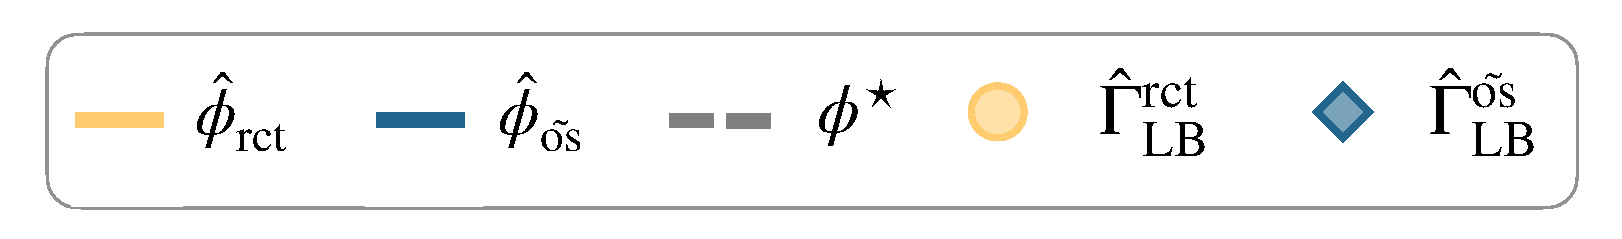
\includegraphics[width=0.9\textwidth]{papers/confounding_test/figures/legend.pdf}\\[0.6ex]
  \begin{subfigure}[b]{0.46\textwidth}
    \centering
    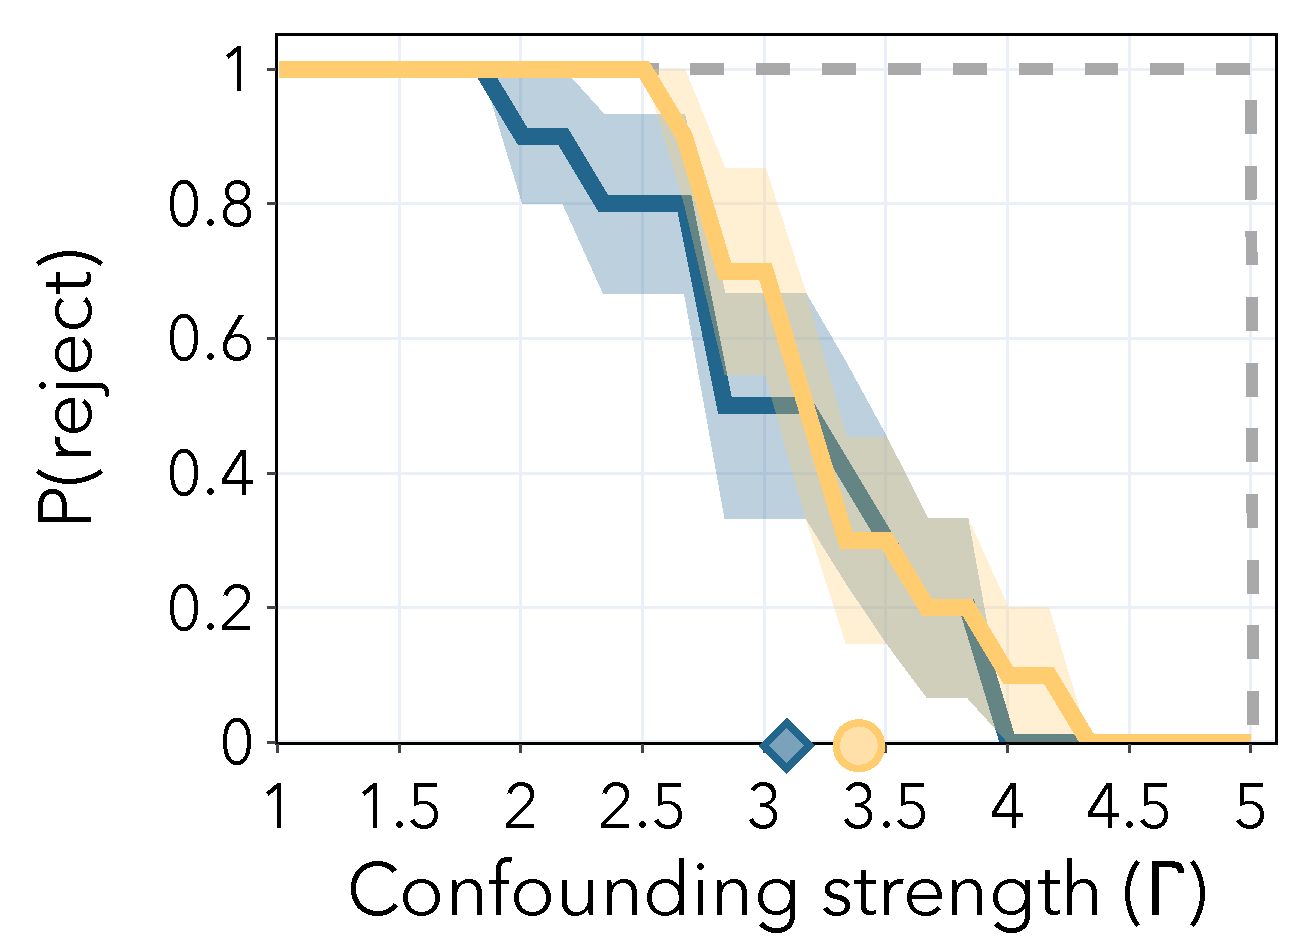
\includegraphics[width=\textwidth]{papers/confounding_test/figures/synthetic_small.pdf}
    \caption{Small sample (\(n_{\mathrm{rct}}=n_{\mathrm{os}}=2{,}000\))}
    \label{fig:confounding-synthetic-small}
  \end{subfigure}
  \hfill
  \begin{subfigure}[b]{0.46\textwidth}
    \centering
    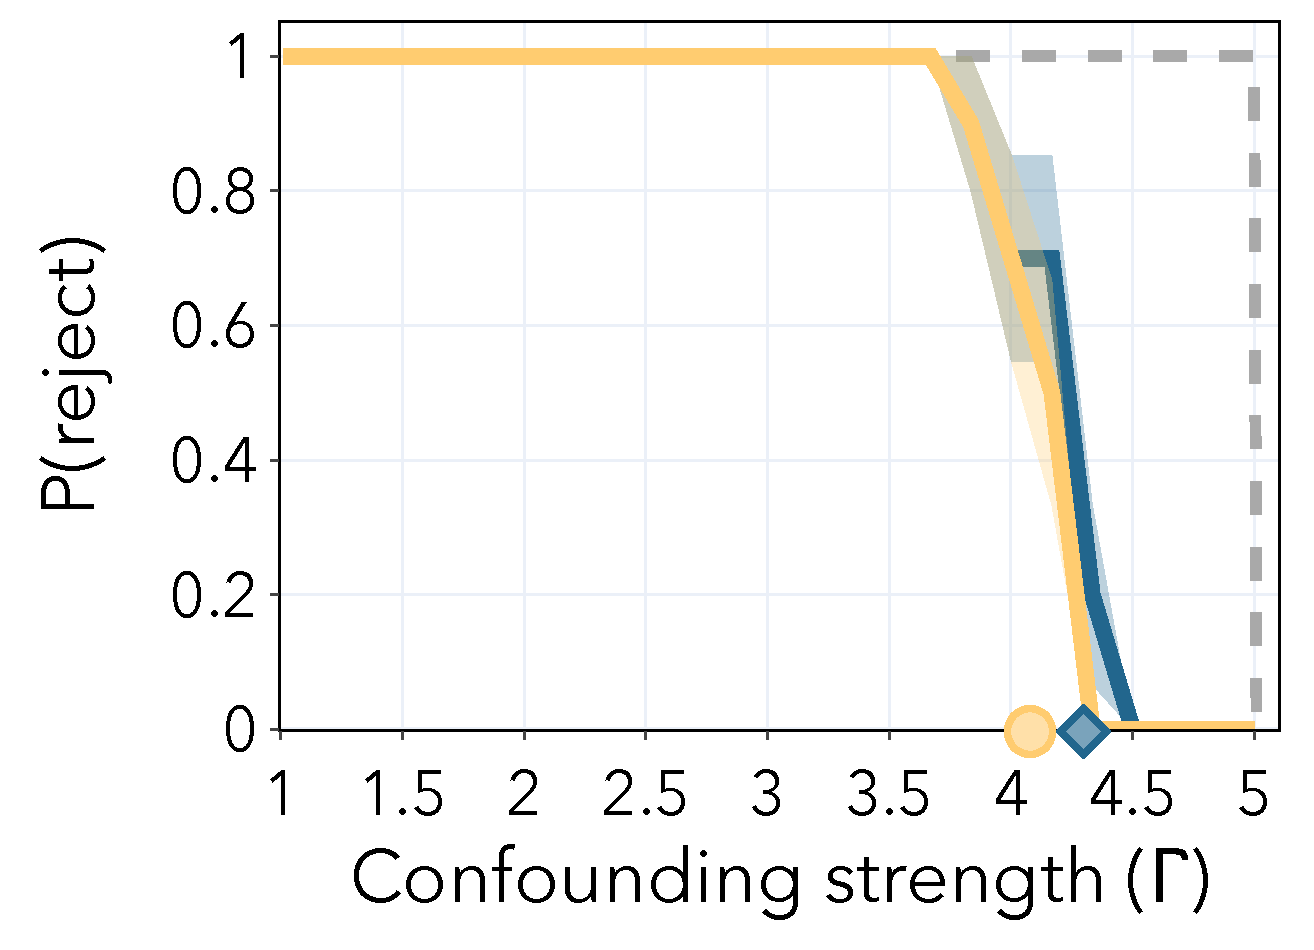
\includegraphics[width=\textwidth]{papers/confounding_test/figures/synthetic_large.pdf}
    \caption{Large sample (\(n_{\mathrm{rct}}=n_{\mathrm{os}}=20{,}000\))}
    \label{fig:confounding-synthetic-large}
  \end{subfigure}\\[0.8ex]
  \begin{subfigure}[b]{0.46\textwidth}
    \centering
    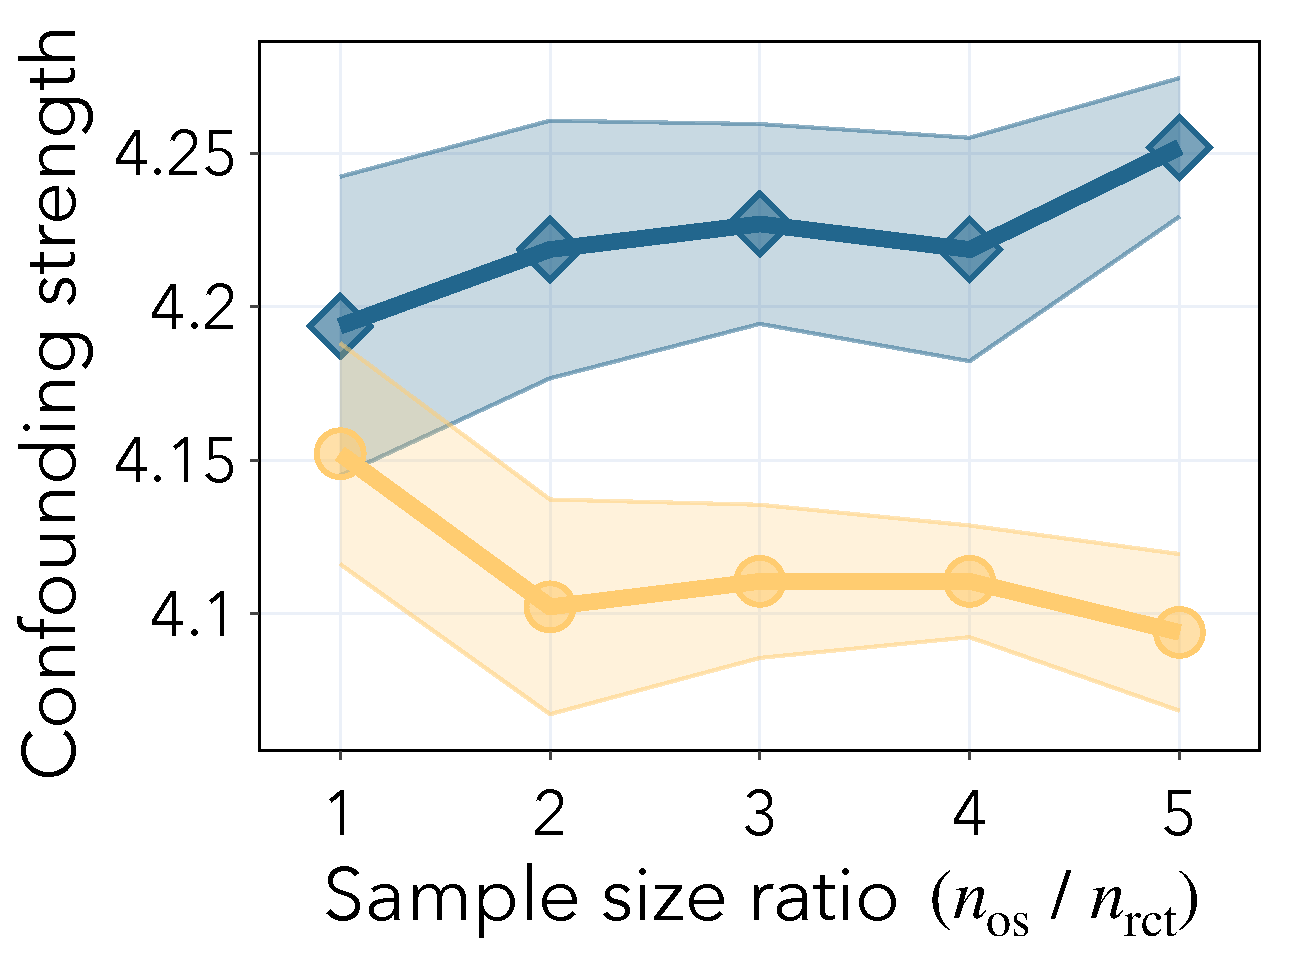
\includegraphics[width=\textwidth]{papers/confounding_test/figures/synthetic_nobs.pdf}
    \caption{Increasing \(n_{\mathrm{os}}\) (\(n_{\mathrm{rct}}=20{,}000\))}
    \label{fig:confounding-synthetic-nobs}
  \end{subfigure}
  \hfill
  \begin{subfigure}[b]{0.46\textwidth}
    \centering
    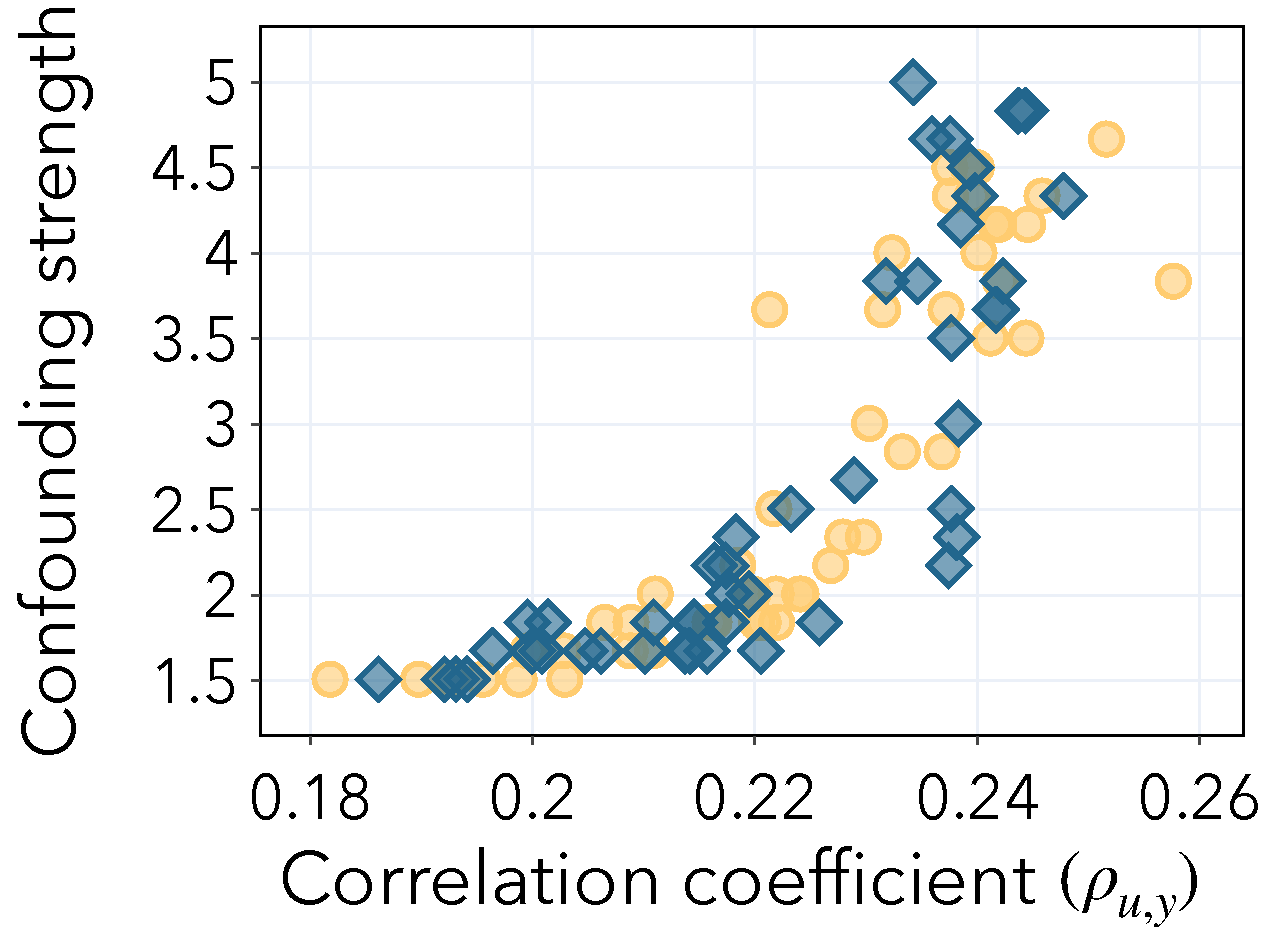
\includegraphics[width=\textwidth]{papers/confounding_test/figures/synthetic_correlation.pdf}
    \caption{Effect of \(\rho_{u,y}\) (\(n_{\mathrm{rct}}=n_{\mathrm{os}}=20{,}000\))}
    \label{fig:confounding-synthetic-correlation}
  \end{subfigure}
  \caption{Finite-sample behavior of the tests and lower bounds on the synthetic benchmark with \(\Gamma^{\star}=5\) and \(\alpha=0.05\). In the legend, \(\phi^{\star}\) denotes the oracle test that rejects whenever \(\Gamma<\Gamma^{\star}\), while \(\widehat{\Gamma}_{\mathrm{LB}}^{\mathrm{rct}}\) and \(\widehat{\Gamma}_{\mathrm{LB}}^{\widetilde{\mathrm{os}}}\) denote the lower bounds obtained from \(\widehat{\phi}_{\mathrm{rct}}\) and \(\widehat{\phi}_{\widetilde{\mathrm{os}}}\). Panels~(a) and~(b) show rejection probabilities and average lower bounds in small- and large-sample regimes; panel~(c) shows lower bounds as \(n_{\mathrm{os}}\) grows; panel~(d) shows lower bounds across varying outcome-confounder correlation \(\rho_{u,y}\).}
  \label{fig:confounding-synthetic-results}
\end{figure}

\begin{figure}[!t]
  \centering
  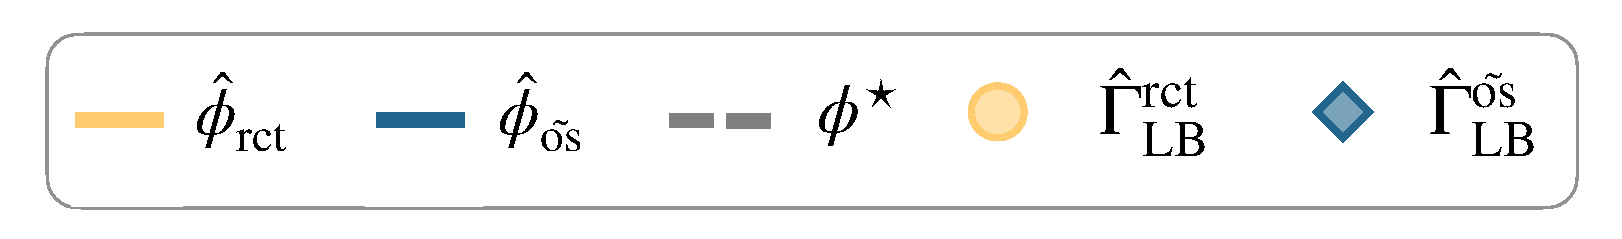
\includegraphics[width=0.9\textwidth]{papers/confounding_test/figures/legend.pdf}\\[0.6ex]
  \begin{subfigure}[b]{0.46\textwidth}
    \centering
    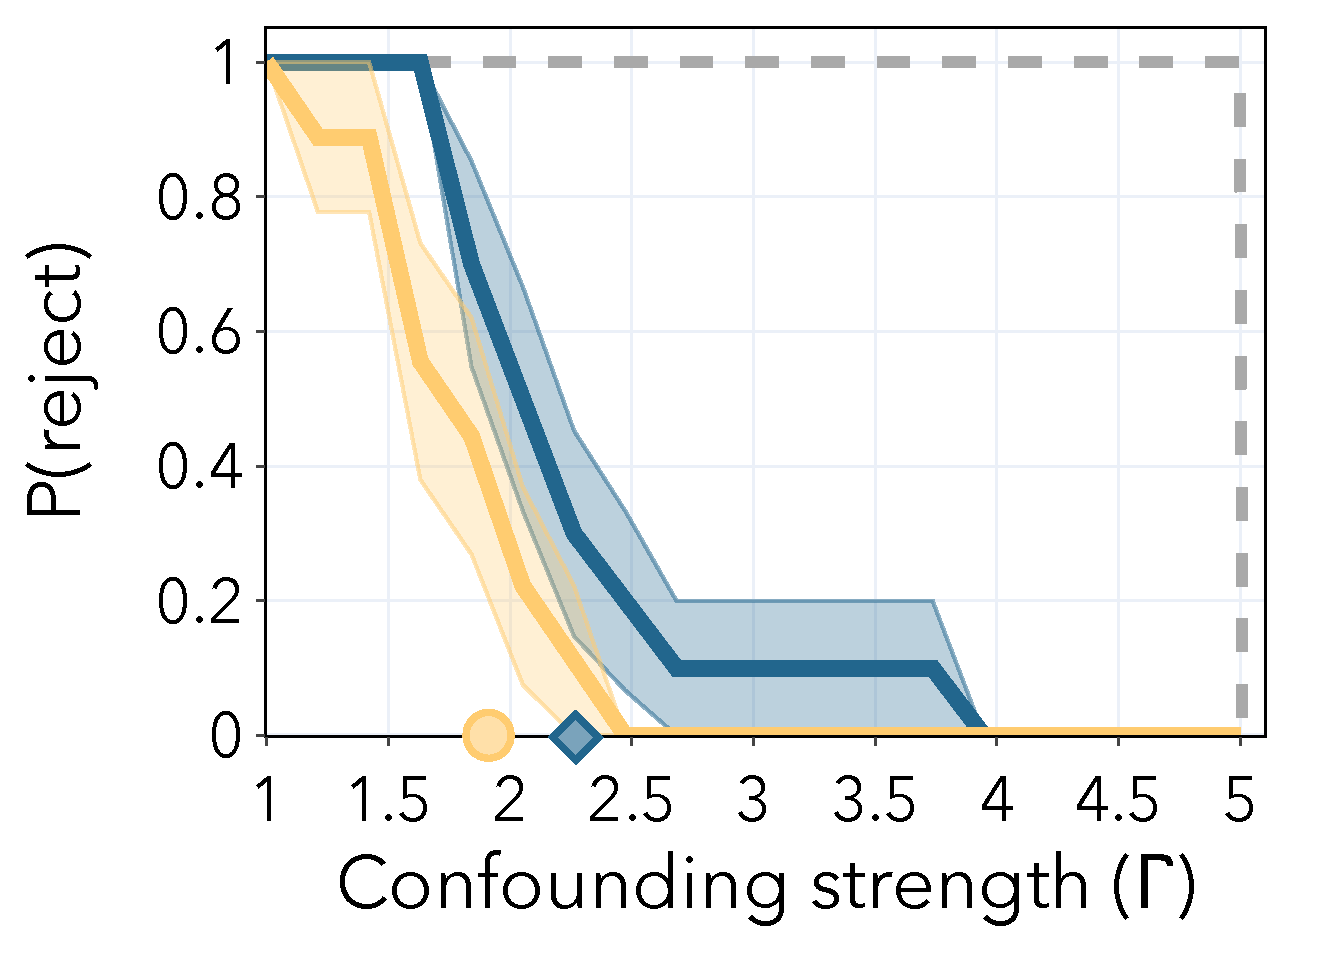
\includegraphics[width=\textwidth]{papers/confounding_test/figures/hillstrom_small.pdf}
    \caption{Small sample (\(n_{\mathrm{rct}}=2{,}300\), \(n_{\mathrm{os}}=6{,}150\))}
    \label{fig:confounding-hillstrom-small}
  \end{subfigure}
  \hfill
  \begin{subfigure}[b]{0.46\textwidth}
    \centering
    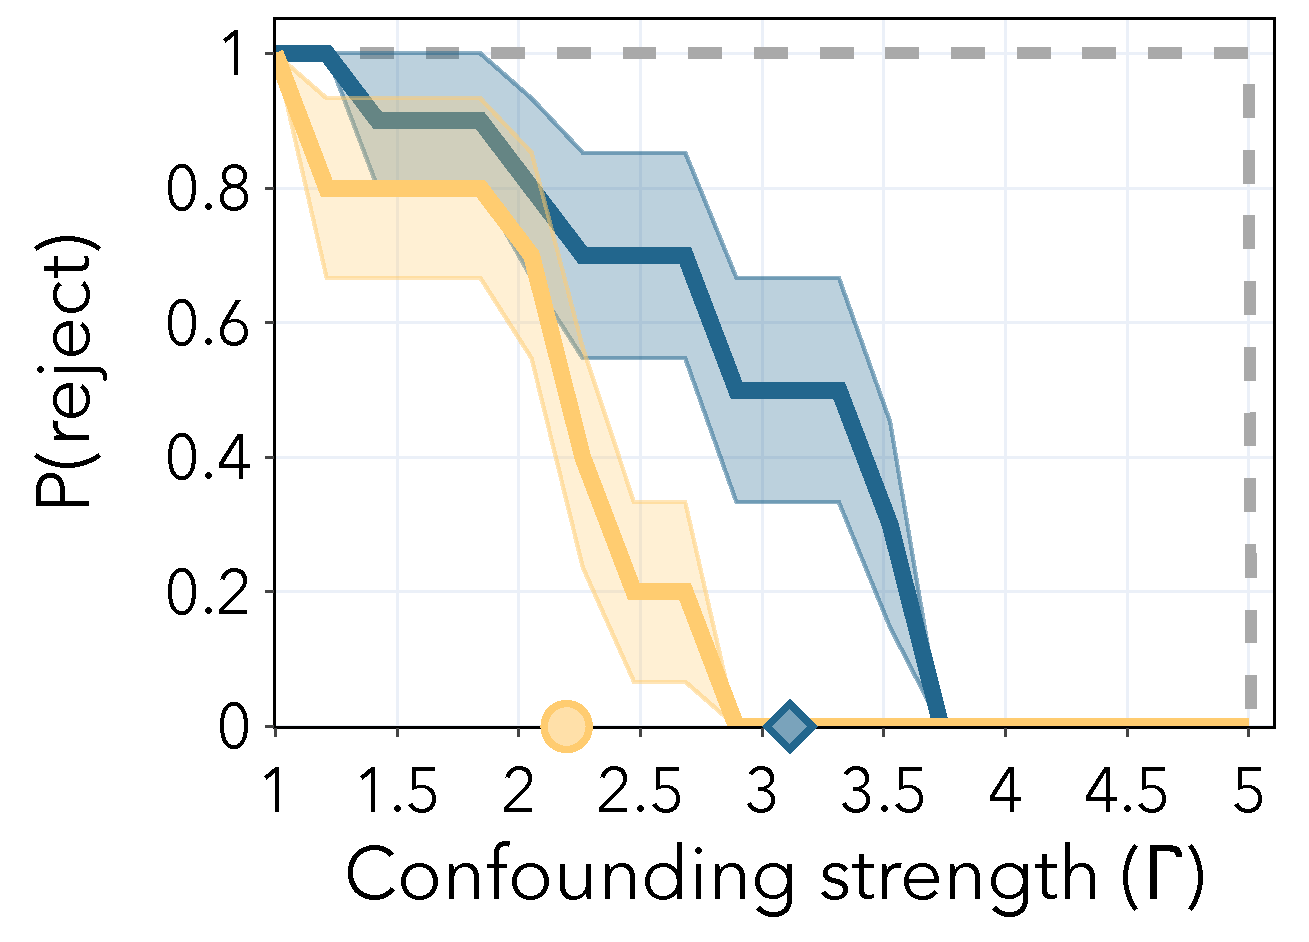
\includegraphics[width=\textwidth]{papers/confounding_test/figures/hillstrom_large.pdf}
    \caption{Large sample (\(n_{\mathrm{rct}}=7{,}680\), \(n_{\mathrm{os}}=20{,}500\))}
    \label{fig:confounding-hillstrom-large}
  \end{subfigure}\\[0.8ex]
  \begin{subfigure}[b]{0.46\textwidth}
    \centering
    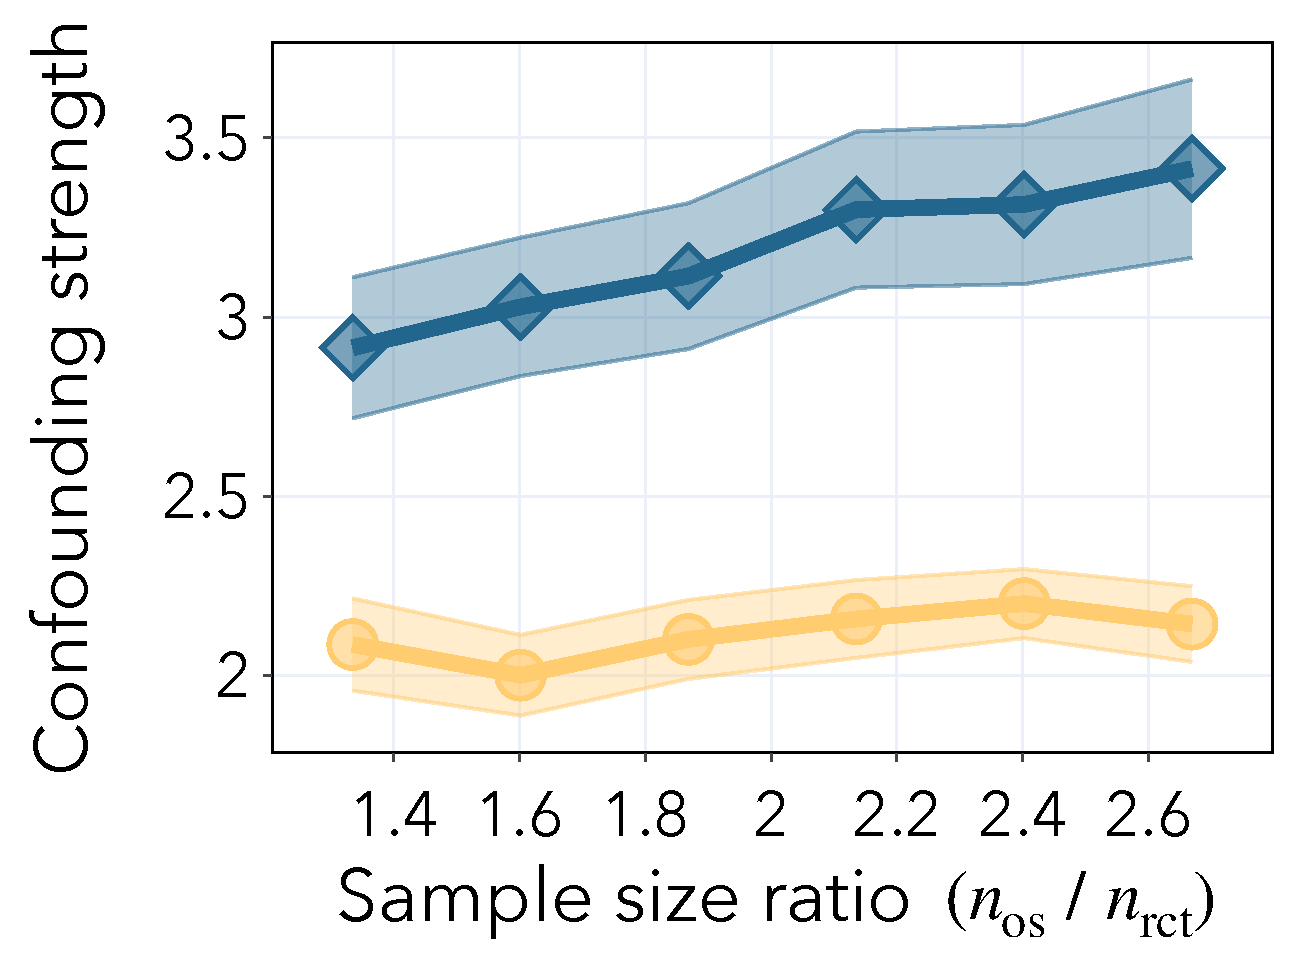
\includegraphics[width=\textwidth]{papers/confounding_test/figures/hillstrom_nobs.pdf}
    \caption{Increasing \(n_{\mathrm{os}}\) (\(n_{\mathrm{rct}}=7{,}680\))}
    \label{fig:confounding-hillstrom-nobs}
  \end{subfigure}
  \hfill
  \begin{subfigure}[b]{0.46\textwidth}
    \centering
    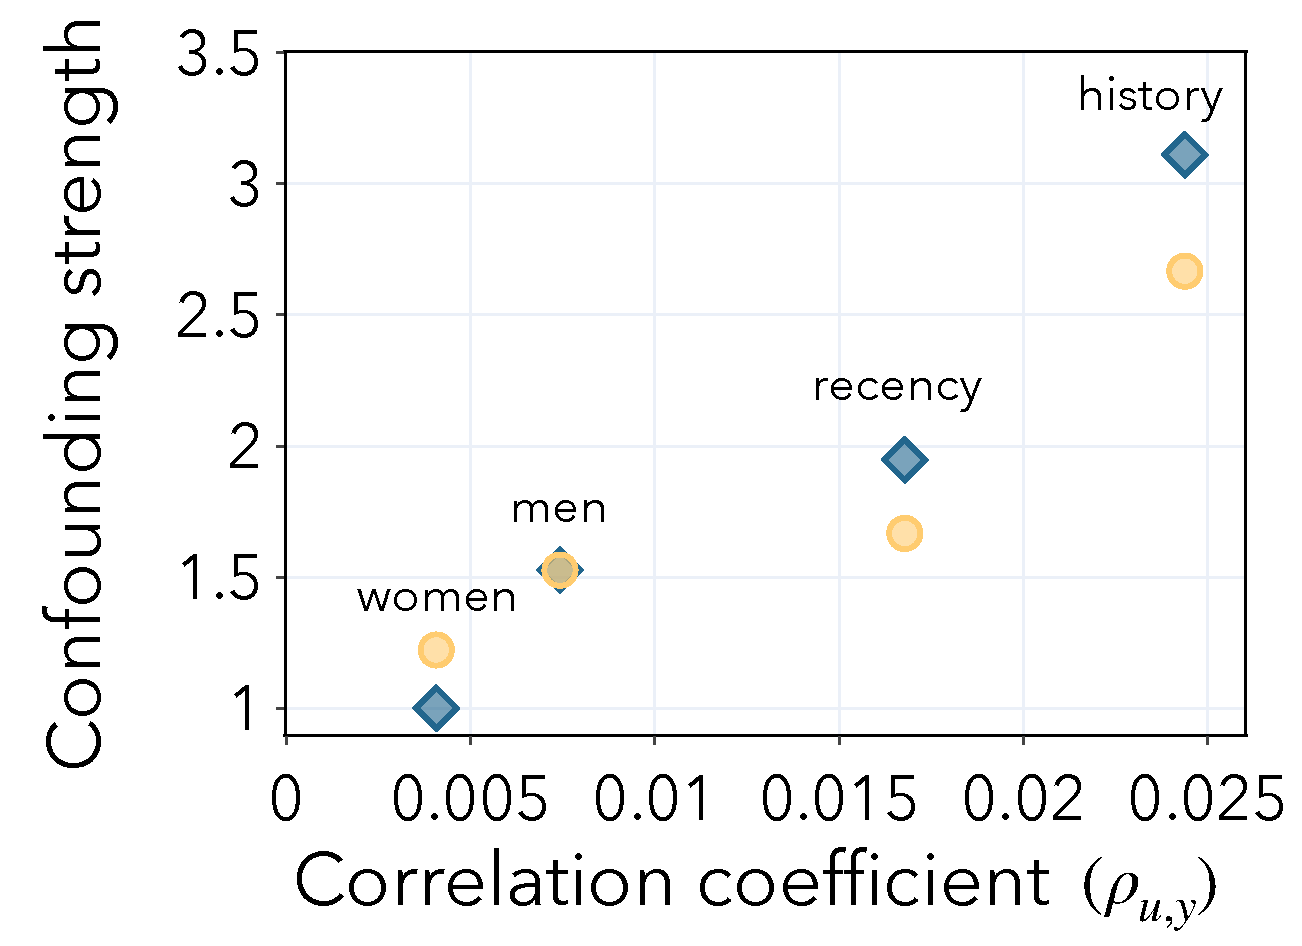
\includegraphics[width=\textwidth]{papers/confounding_test/figures/hillstrom_correlation.pdf}
    \caption{Effect of \(\rho_{u,y}\) across confounders}
    \label{fig:confounding-hillstrom-correlation}
  \end{subfigure}
  \caption{Finite-sample behavior of the tests and lower bounds on the semi-synthetic Hillstrom benchmark with \(\Gamma^{\star}=5\) and \(\alpha=0.05\), using ``history'' as the hidden confounder in panels~(a)--(c). Legend symbols match Figure~\ref{fig:confounding-synthetic-results}. Panels~(a) and~(b) report rejection probabilities and average lower bounds in small- and large-sample regimes; panel~(c) shows lower bounds as \(n_{\mathrm{os}}\) grows; panel~(d) compares lower bounds across hidden covariates with different \(\rho_{u,y}\).}
  \label{fig:confounding-hillstrom-results}
\end{figure}

Figures~\ref{fig:confounding-synthetic-results} and~\ref{fig:confounding-hillstrom-results} summarize the synthetic and semi-synthetic findings. In the rejection-probability panels (Figures~\ref{fig:confounding-synthetic-small}, \ref{fig:confounding-synthetic-large}, \ref{fig:confounding-hillstrom-small}, and~\ref{fig:confounding-hillstrom-large}), both tests remain valid in these finite-sample settings: they do not reject at inflated rates for strengths larger than \(\Gamma^{\star}\).

\subsection{How Does Sample Size Affect Power?}

Comparing the small- and large-sample rejection curves (Figures~\ref{fig:confounding-synthetic-small}--\ref{fig:confounding-synthetic-large} and~\ref{fig:confounding-hillstrom-small}--\ref{fig:confounding-hillstrom-large}) shows that statistical power substantially improves in the large-sample regime. In both the synthetic and Hillstrom settings, larger samples produce sharper transitions around \(\Gamma^{\star}\), leading to more informative lower bounds. Figures~\ref{fig:confounding-synthetic-nobs} and~\ref{fig:confounding-hillstrom-nobs} also show that the two tests respond differently to additional observational data. The restricted-observational test \(\widehat{\phi}_{\widetilde{\mathrm{os}}}\) benefits more from a larger observational study because its sensitivity interval is estimated on the restricted observational target population. This is relevant for post-marketing surveillance: increasing randomized-trial sample sizes is often constrained by the logistics of running additional experiments, whereas observational cohorts can grow through electronic health records, insurance claims, and newly exposed individuals.

\subsection{When Is the Lower Bound Informative?}

The tests are somewhat conservative when \(\Gamma\) is close to \(\Gamma^{\star}\), which can lead to a loose lower bound estimate. This reflects a limitation of the marginal sensitivity model: without additional assumptions on how \(U\) affects \(Y\), a hidden confounder with the same odds-ratio strength can have very different implications for the ATE (see Appendix~\ref{app:confounding-msm-tightness}). To examine this effect directly, Figure~\ref{fig:confounding-synthetic-correlation} evaluates \(\widehat{\Gamma}_{\mathrm{LB}}^{\mathrm{rct}}\) and \(\widehat{\Gamma}_{\mathrm{LB}}^{\widetilde{\mathrm{os}}}\) across \(50\) random draws of the outcome noise variance in \([0,1]\) while holding \(\Gamma^{\star}=5\) fixed, and Figure~\ref{fig:confounding-hillstrom-correlation} varies the hidden covariate \(U\) in Hillstrom. In both benchmarks, higher \(\rho_{u,y}\) correlates with tighter lower bounds for both tests. Conversely, when \(U\) carries little information about the potential outcomes, the lower bound may remain close to one even when \(\Gamma^{\star}\) is larger.

\FloatBarrier

\subsection{Can the Lower Bound Guide Real-World Decisions?}
\label{sec:confounding-real-world}

The Women's Health Initiative (WHI) experiment addresses this question in a real epidemiological setting. Linking back to the post-marketing pipeline, the goal is to show how the lower bound can differentiate between studies with significant confounding and those with negligible confounding. The WHI study included both a randomized trial and an observational study on hormone replacement therapy (HRT) and cardiovascular outcomes \citep{anderson2003implementation}. Historically, the observational study suggested that HRT had a protective effect, while the randomized trial indicated the opposite. This discrepancy was later linked to hidden confounding by time since the start of HRT \citep{vandenbroucke2009hrt}.

To turn the lower bound into a decision rule, we compare it with an observational critical value
\[
  \widehat{\Gamma}_{\mathrm{CT}}
  =
  \inf
  \left\{
    \Gamma:
    0
    \in
    [
      \widehat{\mu}^-_{\Gamma},
      \widehat{\mu}^+_{\Gamma}
    ]
  \right\}.
\]
This critical value is the smallest confounding strength at which the sensitivity interval includes zero, and hence the smallest strength at which the observational treatment-effect conclusion is no longer robust. Similar critical values are commonly used to assess robustness of conclusions drawn from observational data \citep{vanderweele2017sensitivity,jin2023sensitivity}. The most appropriate critical value depends on the scientific context. Since the WHI study satisfies the nested-trial-design criteria, we compute the lower bound using \(\widehat{\phi}_{\widetilde{\mathrm{os}}}\) and write \(\widehat{\Gamma}_{\mathrm{LB}}\) as shorthand for \(\widehat{\Gamma}_{\mathrm{LB}}^{\widetilde{\mathrm{os}}}\) in this subsection and Table~\ref{tab:confounding-whi}. Here we flag the study as practically confounded when
\[
  \widehat{\Gamma}_{\mathrm{LB}}
  >
  \widehat{\Gamma}_{\mathrm{CT}}.
\]
For comparison, we also report the binary decision rule that flags a study whenever \(\widehat{\Gamma}_{\mathrm{LB}}>1\). In contrast to the lower-bound rule, the binary rule flags the observational study if any level of confounding is detected. Experimental details for the WHI analysis are provided in Appendix~\ref{app:confounding-whi-details}.

\begin{table}[!t]
\centering
\caption{WHI evaluation at significance level \(\alpha=0.05\), using \(\widehat{\phi}_{\widetilde{\mathrm{os}}}\) (with \(\widehat{\Gamma}_{\mathrm{LB}}\) denoting \(\widehat{\Gamma}_{\mathrm{LB}}^{\widetilde{\mathrm{os}}}\)). The setting \(t=0\) includes only patients who were not previous users of hormone replacement therapy, while \(t\leq 20\) includes patients with up to 20 years since treatment start. A decision value of \(1\) flags the observational study as confounded.}
\label{tab:confounding-whi}
\begin{tabular}{lcccc}
\toprule
\multirow{2}{*}{Metric} & \multicolumn{2}{c}{Stroke} & \multicolumn{2}{c}{Coronary heart disease} \\
\cmidrule(lr){2-3} \cmidrule(lr){4-5}
& \(t=0\) & \(t\leq 20\) & \(t=0\) & \(t\leq 20\) \\
\midrule
\(\widehat{\Gamma}_{\mathrm{CT}}\) & 1.017 & 1.172 & 1.017 & 1.164 \\
\(\widehat{\Gamma}_{\mathrm{LB}}\) & 1.052 & 1.207 & 1.009 & 1.224 \\
\midrule
Binary rule & 1 & 1 & 1 & 1 \\
Lower-bound rule & 1 & 1 & 0 & 1 \\
\bottomrule
\end{tabular}
\end{table}

Table~\ref{tab:confounding-whi} shows that the lower-bound rule recovers the expected distinction for coronary heart disease. When strong hidden confounding is present in the full observational cohort (\(t\leq 20\)), the procedure flags the study. When the analysis is restricted to participants with \(t=0\), where the major known confounder has been removed, the lower-bound rule does not flag the study, whereas the binary rule still does. This illustrates the practical advantage of distinguishing small and large unobserved confounding rather than flagging any detectable confounding.

For stroke, both rules flag the observational study even after restricting to \(t=0\). This aligns with epidemiological analyses suggesting that additional unobserved confounding factors for stroke may remain even after accounting for time since treatment start \citep{prentice2005combined}. The WHI example therefore illustrates the intended use of the lower bound: it can identify settings where hidden confounding appears practically important while avoiding false alarms in settings where detectable residual confounding is too small to overturn the relevant conclusion.

An alternative way to reach similar conclusions in this example is to test the difference in ATE estimates between the randomized and observational studies. However, the lower-bound approach connects directly to sensitivity analysis: it allows comparing critical values for arbitrarily fine-grained subgroups, up to the individual level via CATE sensitivity bounds, against the same lower bound. In contrast, testing differences in group-level ATE estimates would require a separate test for each subgroup, raising multiple-testing and sample-size concerns.

\FloatBarrier

\section{Chapter Summary}

This chapter introduced a framework for quantifying hidden confounding in observational causal inference by leveraging randomized trials. By combining marginal sensitivity analysis with randomized estimates of target treatment effects, the chapter developed tests for whether unobserved confounding exceeds a specified strength and showed how to invert these tests into an asymptotically valid lower bound on the true confounding strength. The synthetic, semi-synthetic, and WHI experiments show that this lower bound can distinguish negligible from practically important confounding, supporting more reliable causal conclusions from observational data.
